\renewcommand{\myauthor}{Christina Seidner}

Da ein Ziel dieser Diplomarbeit die Möglichkeit, bereits gespielte Spiele zu analysieren, ist, braucht es ein Webinterface. Dieses besteht aus drei Komponenten: Website (Frontend), Server (Backend) und Datenbank. Alle drei sind eng miteinander verbunden und arbeiten zusammen, um eine reibungslose Benutzererfahrung zu gewährleisten.

\subsection{Entwicklungsumgebung und Software-Architektur}
Die Website ist die Benutzeroberfläche, über die die Nutzer mit dem System interagieren. Sie bietet Funktionen wie die Anzeige von bereits gespielten Spielen, die Erstellung von neuen Nutzern und das Spielen neuer Spiele. 

\subsubsection{Entwicklungs-Tools}
Für die Entwicklung des Webinterfaces wurden verschiedene Tools und Technologien verwendet. Dazu gehören:
\begin{itemize}
    \item Visual Studio Code: Dieser Code-Editor wurde für die Entwicklung des Backends und des Frontends verwendet. 
    \item Nano: Wurde auf dem Server verwendet, um Dateien direkt zu bearbeiten.
    \item Git: Wurde für die Versionskontrolle und Zusammenarbeit verwendet, um den Code effizient zu verwalten und Änderungen nachzuverfolgen.
    \item Python: Die Hauptprogrammiersprache für die Backend-Entwicklung.
    \item Flask: Ein leichtgewichtiges Webframework für Python, das gut mit den anderen Komponenten zusammenarbeitet.
    \item MariaDB: Ein relationales Datenbankmanagementsystem, das zur Speicherung der Spieldaten verwendet wird.
    \item HTML/CSS/JavaScript: Für die Gestaltung und Funktionalität des Frontends.
\end{itemize}

\subsubsection{Ordnerstruktur}
\begin{itemize}
    \item frontend/: Dieser Ordner enthält alle Dateien, die man für die Gestaltung der Website braucht. Dazu gehören die HTML-Dateien (index.html, Benutzereingabe.html, Schachbrett.html, Spielanalyse.html und weiterleitung.html), die CSS-Dateien (styles.css, maincss.css), die JavaScript-Datei (api.js), ico-Datei für das Logo (favicon.ico) und die Bilder (schachbrett.jpg und die Schachfiguren).
    \item backend/: Dieser Ordner enthält alle Dateien, die im Hintergrund laufen. Das sind die Python-Dateien (__init__.py, backend.py, receive.py und wsgi.py) und die pgn-Dateien für die bereits gespielten Spiele.
\end{itemize}

\subsubsection{Der Fluss der Daten}
Die Daten fließen zwischen dem Frontend und dem Backend über API-Aufrufe.
Ein Beispiel: \\
\texttt{Wenn der Nutzer auf schachbrett.html einen Zug macht, registriert ein JavaScript-Event-Listener diese Aktion und bereitet die Daten für den POST-Request an den /save_game-Endpunkt vor. Der Server empfängt diese Daten, verarbeitet sie und speichert sie in der Datenbank. Sobald die Daten erfolgreich gespeichert wurden, sendet der Server eine Bestätigung zurück an das Frontend, das dann die Benutzeroberfläche entsprechend aktualisiert, um den neuen Spielstand anzuzeigen.}


\subsection{Bereitstellungsprozess}
\subsubsection{Der Ursprung}
Am Anfang wurde die Website lokal auf dem persönlichen Laptop entwickelt. Alle Funktionen wurden implementiert und getestet, um sicherzustellen, dass sie wie erwartet funktionieren. Der Laptop diente sozusagen als vorübergehender Server. Erst danach wurde die Website auf den Debian-Server der Schule übertragen. 
Dafür wurden alle benötigten Dateien in das GitHub-Repository hochgeladen und von dort aus auf den Server geklont. 
Auf einem Windows-PC funktioniert das mit \\
\texttt{git clone https://github.com/nextmove-interactive-chessboard/documentation.}

\subsubsection{SSH-Key-Authentifizierung}
Da der Server in Linux-Debian läuft, kann das GitHub-Repository nicht genauso geklont werden, da es aus Sicherheitgründen abgeschafft wurde.
Wenn man es trotzdem versucht, bekommt man die Fehlermeldungen \\
\texttt{remote: Password authentication is not supported.} \\
\texttt{fatal: Authentication failed}


\begin{figure}[htbp]
    \centering
    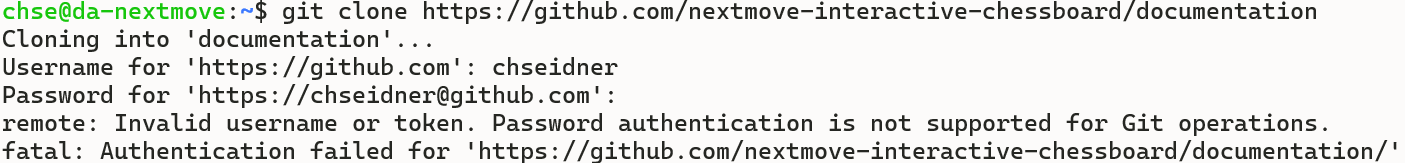
\includegraphics[width=1\textwidth]{figures/gitcloneFalsch.png}
    \caption{Fehlerhafte Git-Clone-Operation}
    \label{fig:gitcloneFalsch}
\end{figure}

\newpage
Daher muss mit dem Befehl \\
\texttt{ssh-keygen -t ed25519 -C "cseidner@tsn.at"} \\
ein ssh-key-Paar angelegt werden, um Zugriff auf das Repository zu bekommen.
Nur, wer den privaten Schlüssel besitzt, kann auf das Repository zugreifen. Dieser bleibt auf dem Server, während der öffentliche Schlüssel in GitHub hinterlegt wird.


\begin{figure}[htbp]
    \centering
    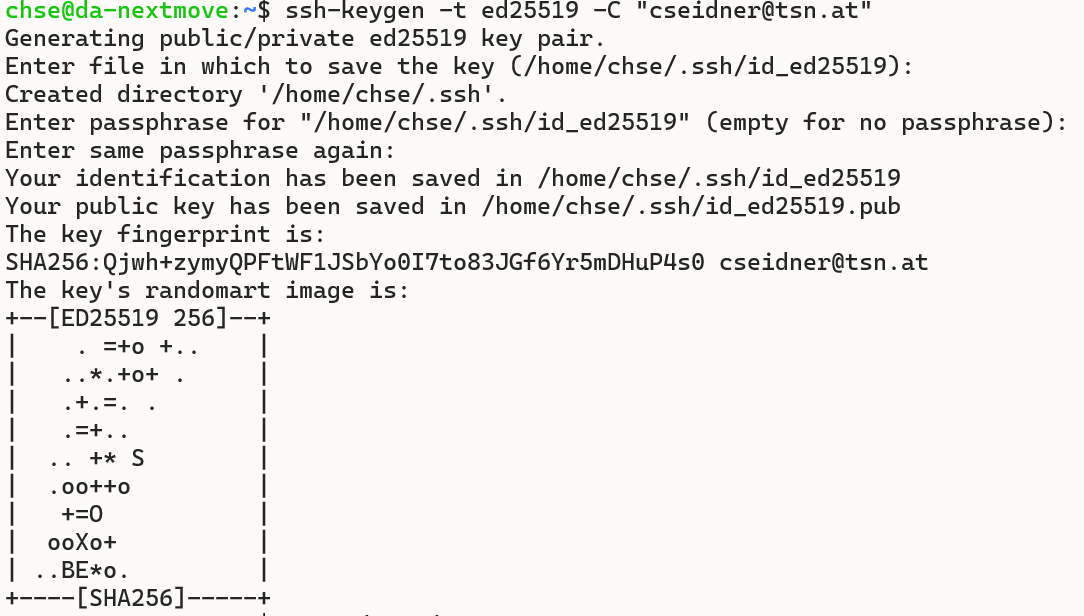
\includegraphics[width=1\textwidth]{figures/sshkey.png}
    \caption{SSH-Key-Generierung}
    \label{fig:sshkey}
\end{figure}

Nun kann der key mit dem Befehl \\
\texttt{cat \string~\string/.ssh/id\_ed25519.pub} \\
angezeigt werden:

\begin{figure}[htbp]
    \centering
    
\includegraphics[width=1\textwidth]{figures/sshkey2.png}
    \caption{SSH-Key-Anzeige}
    \label{fig:sshkey2}
\end{figure}

\newpage
Diesen Key fügt man nun in GitHub unter \\
\texttt{Settings $\rightarrow$ SSH and GPG keys $\rightarrow$ New SSH key} \\
ein. Dieser ssh-key heißt ssh Server (Debian). 

Um jetzt neu klonen zu können, muss die ssh-Konfiguration gegebenenfalls erneuert werden. 

Mit \\
\texttt{eval "\$(ssh-agent -s)"} \\
\texttt{ssh-add \string~\string/.ssh/id\_ed25519} \\
kann überprüft werden, ob der neu erstellte ssh-key tatsächlich aktiv geladen ist. 

Nachdem eine ssh-Konfiguration \texttt{nano \string~\string/.ssh/config} mit dem Inhalt \\
\texttt{Host github.com} \\
\texttt{HostName github.com} \\
\texttt{User git} \\
\texttt{IdentityFile \string~\string/.ssh/id\_ed25519} \\
\texttt{ProxyCommand none} \\

angelegt wurde, müssen noch die Ordnerrechte eingeschränkt werden, damit die ssh-Verbindung nicht alles blockiert: \\
\texttt{chmod 700 \string~\string/.ssh} \\
\texttt{chmod 600 \string~\string/.ssh/id\_ed25519} \\
\texttt{chmod 644 \string~\string/.ssh/id\_ed25519.pub}\\

\newpage
\subsubsection{Deployment}
Nun kann das Repository mit dem ssh-Link geklont werden. Dieser liegt in GitHub unter \texttt{Code $\rightarrow$ SSH}. \\

\begin{figure}[htbp]
    \centering
    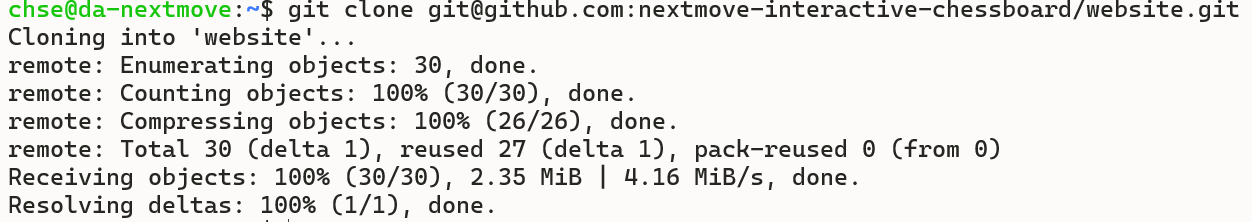
\includegraphics[width=1\textwidth]{figures/gitcloneRichtig.png}
    \caption{Erfolgreiche Git-Clone-Operation}
    \label{fig:gitcloneRichtig}
\end{figure}

\subsection{Datenbank-Design und Implementierung}

\subsection{Server-Konfiguration}

\subsection{Backend-Logik und Socket-Kommunikation}



\newpage
\subsubsection{Frontend}
Zum Frontend der Website gehören alle Elemente, die der Nutzer direkt sieht und mit denen er interagiert. Dazu gehören alle visuelle Elemente.

\subsubsection{Backend}
Das Backend ist der Teil im Hintergrund der Website, der die Logik und die Funktionalität bereitstellt. Es verarbeitet die Anfragen der Nutzer, kommuniziert mit der Datenbank und stellt die benötigten Informationen bereit. Das Backend ist entscheidend für die Funktionalität der Website und sorgt dafür, dass alles reibungslos funktioniert.

Die Implementierung des Backends erfolgt in Python. 

Die Codestruktur sieht wie folgt aus:
\begin{itemize}
    \item backend.py: Dies ist die Hauptdatei, die den Server startet und die Routen definiert.
    \begin{scriptsize}
    \begin{lstlisting}[style=Python, language=Python, captionpos=b, stepnumber=5, caption = {Backend-Implementierung}]
        app = Flask(__name__)
        CORS(app)  

        db_config = {
            "host": os.getenv("DB_HOST", "localhost"),
            "user": os.getenv("DB_USER", "Christina"),
            "password": os.getenv("DB_PASSWORD", "ChrissiNext"),
            "database": os.getenv("DB_NAME", "NextMove"),
        }

        @app.route('/save_game', methods=['POST'])
        def save_game():
            data = request.json  
                        
            query = "INSERT INTO spiele (user_id, gegner_name, ergebnis, pgn_daten) VALUES (%s, %s, %s, %s)"
            cursor.execute(query, (user_id, gegner, ergebnis, pgn))
            
            conn.commit()

    
        @app.route('/get_games/<int:user_id>', methods=['GET'])
        def get_games(user_id):
            cursor = conn.cursor(dictionary=True)
            query = "SELECT * FROM spiele WHERE user_id = %s"
            cursor.execute(query, (user_id,))
            games = cursor.fetchall()
    \end{lstlisting}
    \end{scriptsize}

    \item wsgi.py: Diese Datei dient als Einstiegspunkt für den WSGI-Server, der die Anwendung bereitstellt.
    
    \begin{scriptsize}
    \begin{lstlisting} [style=Python, language=Python, captionpos=b, stepnumber=5, caption = {WSGI-Server-Einstiegspunkt}]
        from backend import app

        if __name__ == "__main__":
            app.run()
    \end{lstlisting}
    \end{scriptsize}
\end{itemize}

\subsection{Datenbank}
Die Datenbank dient als Speicher für alle relevanten Informationen, die vom System verarbeitet werden. Dazu gehören Informationen über die Nutzer, die gespielten Spiele, die Ergebnisse und andere relevante Daten. Die Datenbank ermöglicht es dem Server, schnell auf Anfragen zu reagieren und die benötigten Informationen bereitzustellen.

\subsection{Server}
Der Server dient als zentrale Steuereinheit, die die Kommunikation zwischen der Website und der Datenbank koordiniert. Er verarbeitet die Anfragen der Nutzer und stellt die entsprechenden Daten aus der Datenbank bereit.
Verwendet wird hier ein Linux Debian Server der Schule. 

\begin{figure}[htbp]
    \centering
    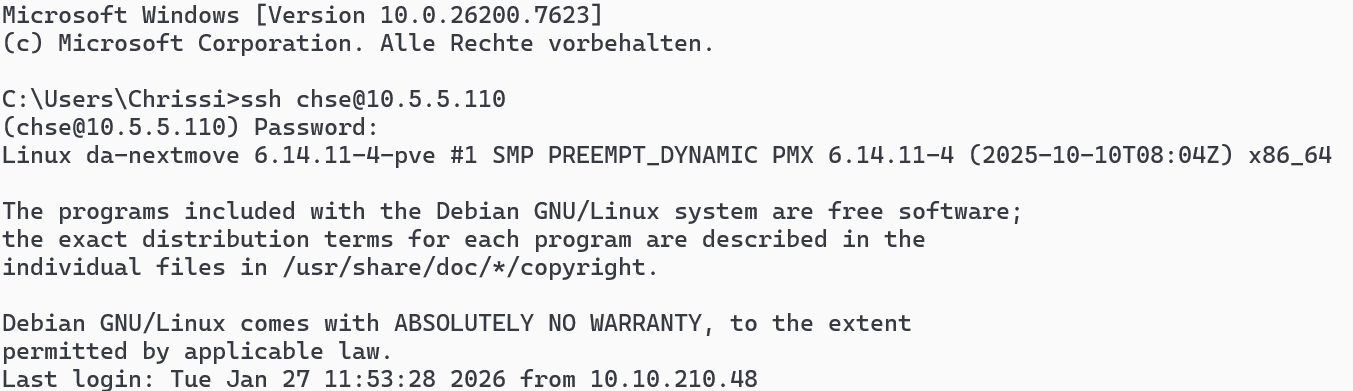
\includegraphics[angle=90, width=0.8\textwidth]{figures/Debian.PNG}
    \caption{Debian-Server.}
    \label{fig:Debian}
\end{figure}